\renewcommand\appendixname{Anhang}
\renewcommand\appendixpagename{Anhang}
\renewcommand\appendixtocname{Anhang}

\lohead{}

% Anhang Seite ohne Kopf- & Fußzeile
\appendix
\begingroup
\makeatletter
\let\ps@plain\ps@empty
\appendixpage
\makeatother
\endgroup

% Anhänge
\chapter{Zeitaufzeichnung}
\chapter{Persönlicher Anhang 1}
\label{cha:anhang}

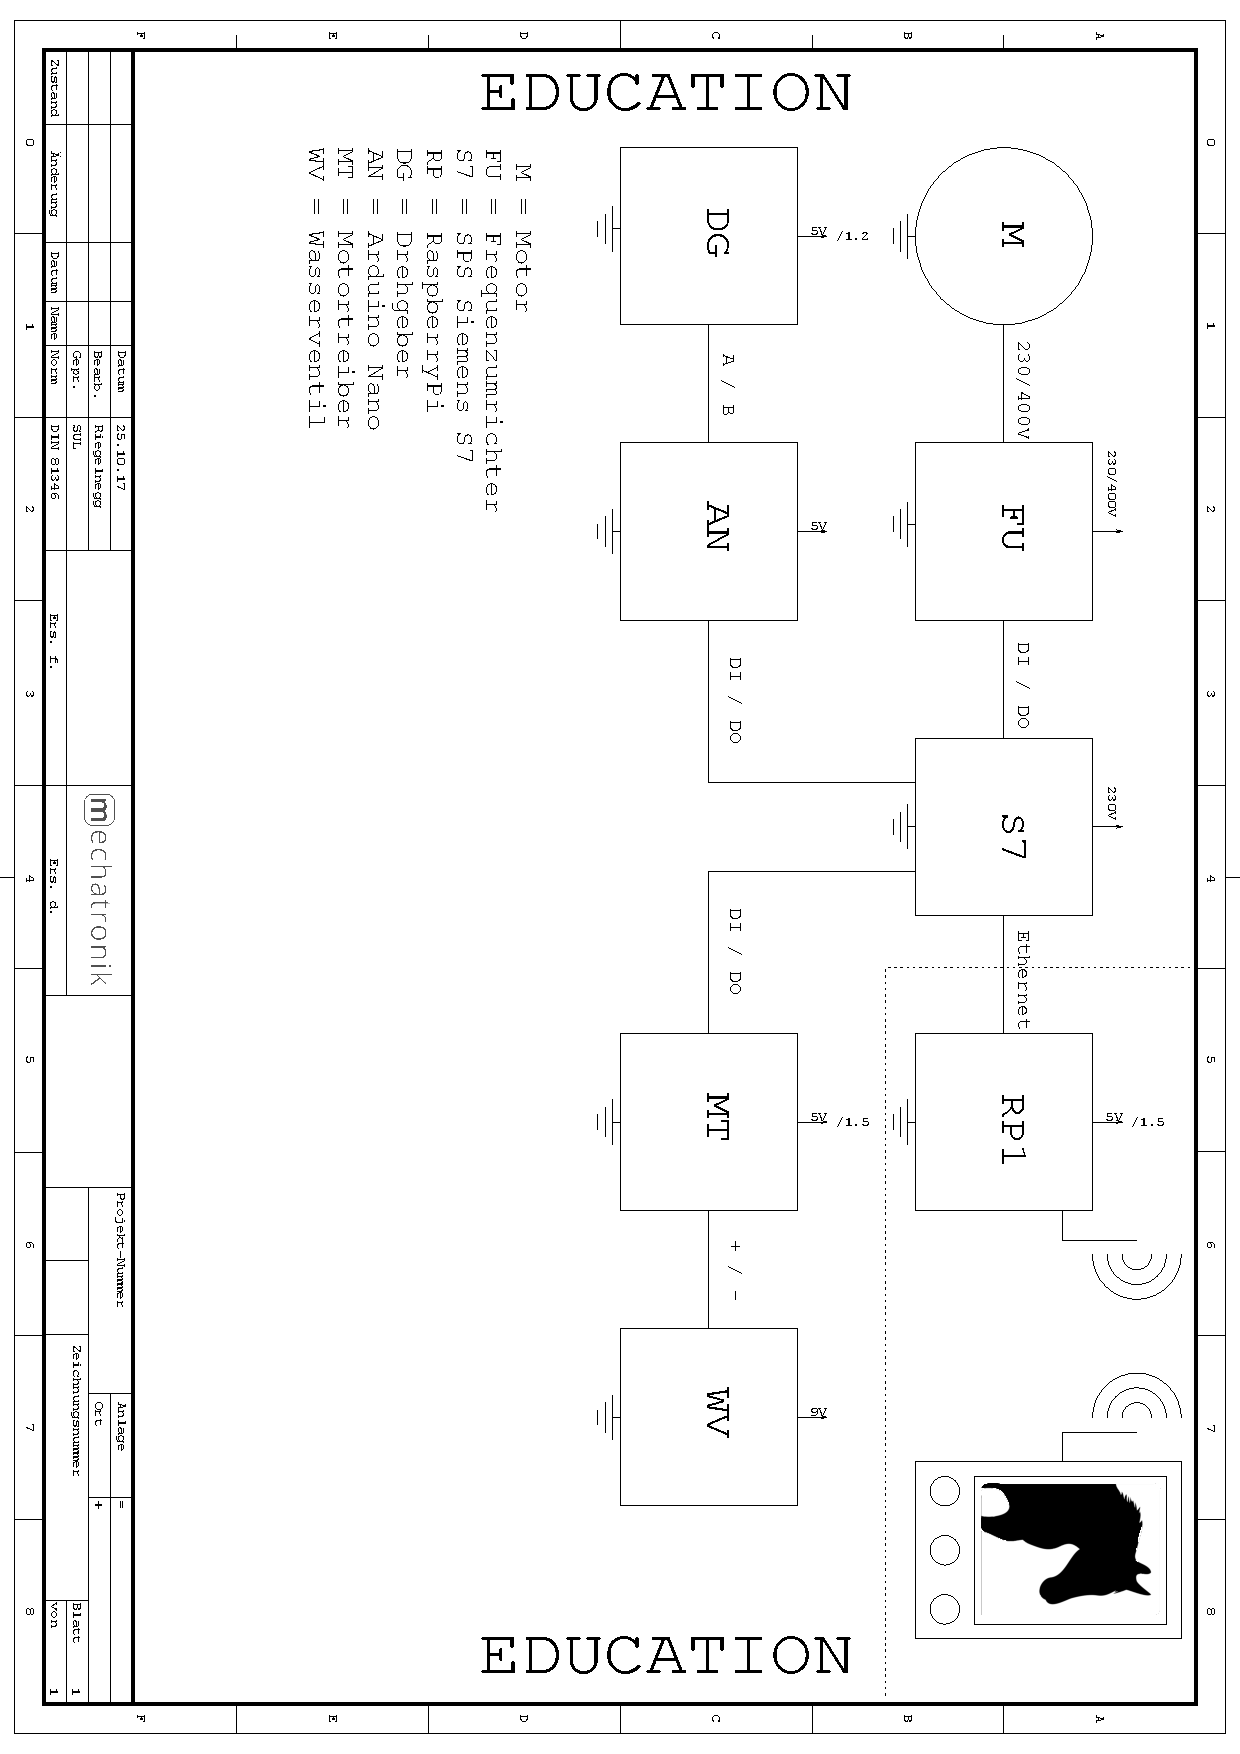
\includegraphics[scale=0.86]{fig/Blockschaltbild1}

\markboth{}{}	%end chapter

\bibliography{Literaturverzeichnis}
\bibliographystyle{unsrt}

\chapter{Abkürzungsverzeichnis}
\begin{acronym}
%Abkürzung hinzufügen: \acro{Kürzel}{Ausgeschrieben}
	\acro{FU}{Frequenzumrichter}
	\acro{ISR}{Interrupt Service Routine}
	\acro{UART}{Universal Asynchronous Receiver and Transmitter}
\end{acronym}

\listoffigures
\listoftables
\lstlistoflistings